\thispagestyle{empty}
\newgeometry{margin=1in}
\begin{center}
{
    \large
    Московский государственный университет имени М. В. Ломоносова\par
    факультет вычислительной математики и кибернетики\par
    кафедра алгоритмических языков\par
}
\par
\end{center}

\vspace{10mm}
\begin{flushright}
%На правах рукописи

{\sl}%УДК xxx.xxx}
\end{flushright}

\begin{center}
%\vspace{10mm}
%{%\small
%Специальность 010200
%
%<<Прикладная математика и информатика>>
%}

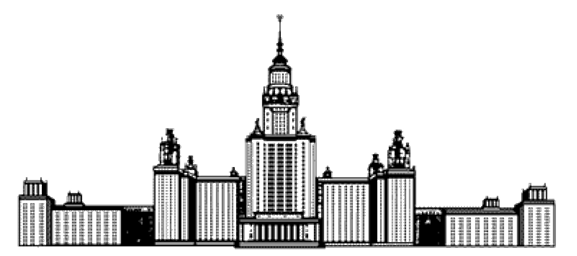
\includegraphics[width=\linewidth]{images/logo}

\vspace{25mm}
Курсовая работа

\vspace{5mm}
{
    \bf \large
    Библиотека для морфологического анализа \\ свободнообразуемых слов русского языка
    \par
}

\end{center}

\vspace{10mm}
\begin{flushright}
Выполнил: студент 324 группы

Гончаренко Евгений Евгеньевич

\vspace{10mm}
Научный руководитель: к.ф.-м.н., доцент

Головин Игорь Геннадьевич
\end{flushright}

\vspace{5mm}
\begin{center}
{Москва 2022}
\end{center}

\newpage
